\chapter{The C-score: where the departures sit}\label{ch:cscore}

\section{Two specimens with the same $A$}

$A$ is an average over a cell's identity sites. Two specimens can read the same $A$ with very different patterns underneath:
a small departure spread evenly over every site, or a large departure concentrated in a few regions of the genome. The second
is what a clone, a deletion or a regional failure of maintenance would leave. The C-score reads that difference, on the same
gauge: healthy is 1.

\section{The residual map}

For each identity site, in genome order, the chain computes how far this specimen's entropy sits from the healthy cell's,
in units of the healthy spread at that site:
\begin{equation}
  z_i=\frac{H(\beta_i)-H(\mathrm{ref}_i)}{s_i},
  \label{eq:z}
\end{equation}
with $\mathrm{ref}_i$ the healthy neutrophil mean entropy at that site (isolated cells) or the person's own expectation
$H(e_i)$ (whole blood), and $s_i$ the shrunken standard deviation of $H$ across the six reference arrays. The map is the cell's
own sky: only measured sites, placed by genome position, nothing interpolated. \derived{} (the construction)

\section{The score}

Consecutive runs of 10 sites are averaged (blocks of 50 until 2026-10-09). If the departures are scattered at random, the block means vary as $1/\sqrt{10}$
of the site values; if they cluster, the block means vary more. The clustering statistic is
\begin{equation}
  c=\frac{\mathrm{var}\left(\sqrt{10}\;\overline{z}_{\rm block}\right)}{\mathrm{var}(z)},\qquad
  C=\frac{c}{c_{\rm healthy}},\qquad c_{\rm healthy}=1.0103,
  \label{eq:C}
\end{equation}
with $c_{\rm healthy}$ the median over the six reference arrays, each read against the other five. \calibrated{} The healthy reference arrays read $C=0.954$--$1.046$; a reading is then tared against healthy arrays run with it ($C_{\rm rel}$) and read against the commissioned band (Status box). A score needs a minimum
number of blocks.

Figure~\ref{fig:p4_cscore_construction} shows the construction on two simulated maps with the same mean departure.

\begin{figure}[htbp]\centering
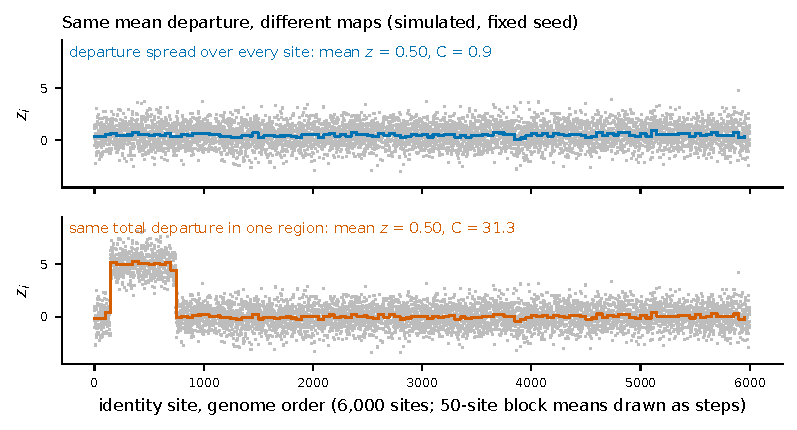
\includegraphics[width=0.95\textwidth]{figures/part6/fig_p4_09_construction.pdf}
\caption{The C-score construction on two simulated residual maps of 6,000 sites (fixed seed). Top: every site moved by $+0.5$ healthy SD.
Bottom: the same total departure placed in one tenth of the genome order. Steps: 50-site block means. $C$ uses the healthy baseline 1.1104.
\calc{} (illustration; no specimen).}
\label{fig:p4_cscore_construction}
\end{figure}

\begin{keybox}[title=Status]
The Met-A C-score is \textbf{commissioned on whole blood} (EPIC v1, 2026-10-15). Blocks of 10 sites; healthy baseline 1.0103 (six
reference arrays, leave one out). The healthy band, 0.877--1.152, was set on 617 healthy arrays from 19 laboratories (DEV_CSCORE_TARE_01_arrays.csv) and is read
one-sided: above 1.152 is a clustered departure, below 0.877 is less clustered than healthy and is not a departure. Three laboratories
that had no part in setting it read 34 of 35, 22 of 23 and 172 of 173 healthy bloods not above it; one person measured twice reads the
same within 0.038 (bar 0.125); clustered loss planted into real healthy arrays is caught every time, scattered loss never. Detection
limit: $C_{\rm rel}=1.5$ at 5\,\% of sites clustered. Isolated neutrophils and real tumors are its next tests. \measured{} The IAM-A C-score, the same map built from per-region held error on
molecules, is defined and not yet built. \openprob
\end{keybox}

Figure~\ref{fig:p4_cscore_readings} and Table~\ref{tab:p4_cscore} give every C-score in the records of chain v3.

\begin{figure}[htbp]\centering
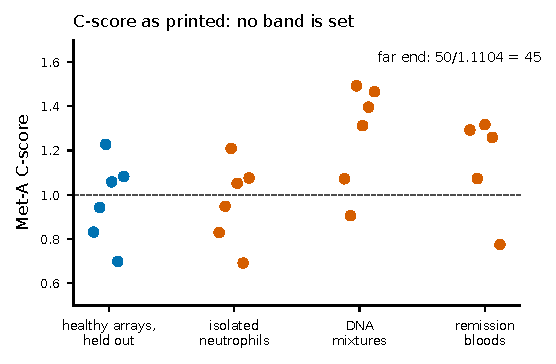
\includegraphics[width=0.62\textwidth]{figures/part6/fig_p4_09_readings.pdf}
\caption{Met-A C-score as printed. Blue: the six reference arrays, each against the other five.
Orange: the acceptance run. Both at blocks of 50, before the band was set; the commissioned band (blocks of 10) is in the Status box. \measured}
\label{fig:p4_cscore_readings}
\end{figure}
\begin{table}[htbp]\centering\small
\caption{Met-A C-scores in the records of chain v3 before the band was set (blocks of 50, 2026-10-04); the commissioning tests are in the Status box.}\label{tab:p4_cscore}
\begin{tabular}{@{}p{0.48\textwidth}rrl@{}}\toprule
set & $n$ & $C$ & status \\\midrule
healthy reference arrays, each against the other five & 6 & 0.70--1.23 & \calibrated \\
isolated reference neutrophils, acceptance run & 6 & 0.69--1.21 & \measured \\
DNA mixtures, acceptance run & 6 & 0.91--1.49 & \measured \\
remission bloods, another laboratory & 5 & 0.78--1.32 & \measured \\
far end: every 50-site block moving as one & --- & 45 & \calc \\
\bottomrule
\end{tabular}
\end{table}

\section{Why it matters}

A loss spread thinly across the genome and a loss concentrated in one region can mean different biology, and only the
second is visible as structure. Serial readings of one person (Chapter~\ref{ch:serial}) make the map sharper with every draw,
because a person's own stable regions become their own reference.
